\documentclass[11pt]{scrartcl}
\usepackage{booktabs}
\usepackage{bbding}
\usepackage{settings}

\lhead{MOP 2024 Practise}
\rhead{\begin{CJK}{UTF8}{ipxm} John Maynard
\end{CJK}}
\usepackage{pdfpages}
\begin{document}

\title{\vspace{-2em}\textcolor{bk}{\textbf{BÀI TẬP TỔ HỢP VÀ ĐẠI SỐ}}}

%\subtitle{\vspace{1.5em}{\textbf{\LARGE CAUCHY-SCHWARZ-HOLDER}}}
\author{Phạm Bảo -\begin{CJK}{UTF8}{ipxm} カズマアカリ。\end{CJK}\vspace{-1em}}

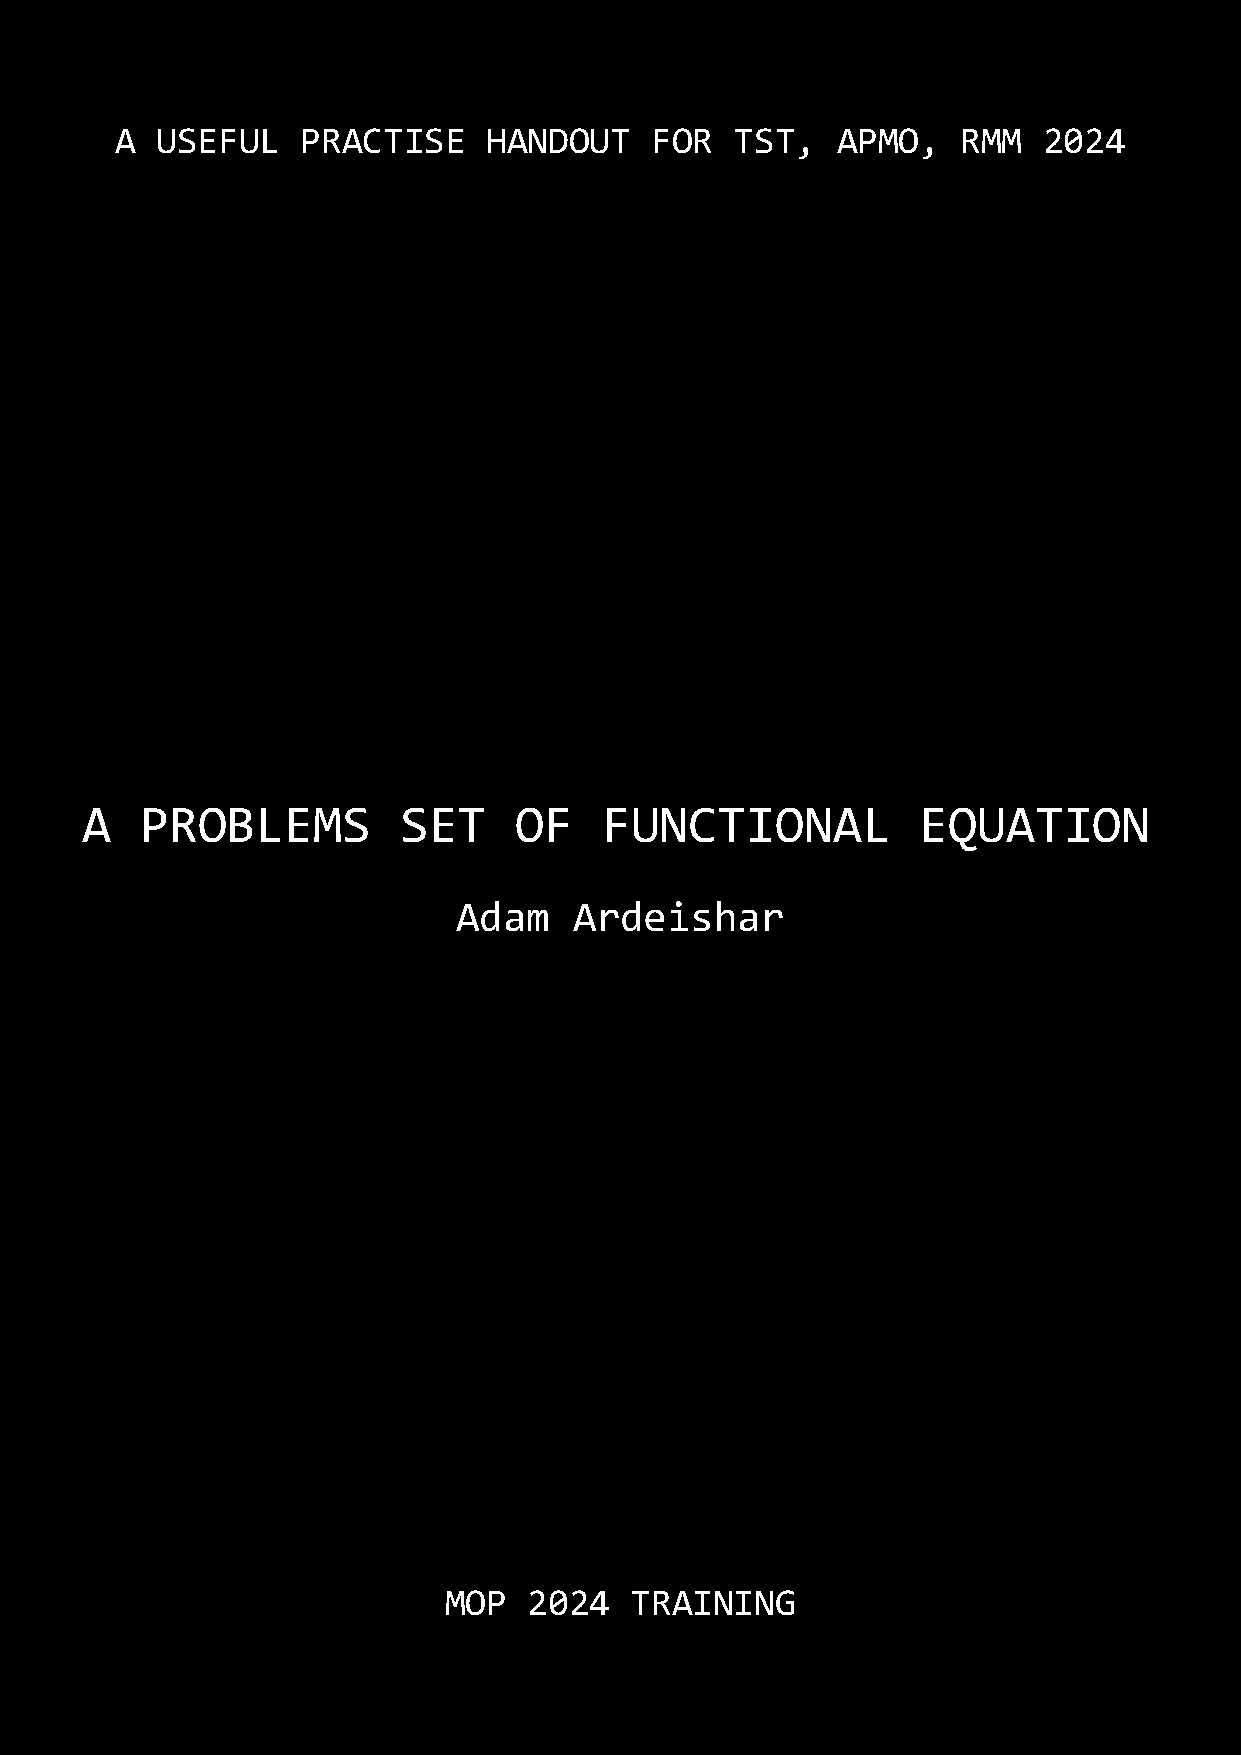
\includepdf[pages=1]{biapt.pdf}
\thispagestyle{empty}


%\subsection*{\Large\textcolor{bk}{ \S 1.1.} Các bất đẳng thức cổ điển}
\newpage
\setcounter{page}{1}
\thispagestyle{plain}
\begin{itemize}[label=, leftmargin=0em, itemsep=0.5em]
    \thispagestyle{plain}

    \section{\huge Phương trình hàm}
    \subsection{\LARGE \textcolor{dk}{Đề bài}}
    \vspace{1em}
    \item \begin{bt}\vocab{(USAMO 2002).}
        Tìm tất cả các hàm số $f: \mathbb{R} \to \mathbb{R}$ thỏa mãn
        \[
           f(x^2 - y^2) = xf(x) - yf(y)
        \]
        với mọi số thực $x,y$.
    \end{bt}
    \begin{sol}
        Ký hiệu $P(x,y)$ chỉ phép thế vào $(?)$ tương ứng. $P(x,0)$ ta được $f(x^2) = xf(x)$. Thay $x \to -x$ ta được $f$ là hàm lẻ. Viết Lại
        \[
            f(x^2 - y^2) = f(x^2) - f(y^2), \xyr
        \]
        Hay $f(x - y) = f(x) - f(y) ,\forall x, y \geq 0$. Thay $x \to x + y$ ta được $f(x) + f(y) = f(x + y), \forall x,y \geq 0$. Mặt khác lại có 
        \[
            -f(x) - f(y) = -f(x + y) \lra f(-x) + f(-y) = f(-x-y),\forall x,y \geq 0
        \]
        Suy ra $f$ cộng tính trên $\bb{R}$. Thế nên với mọi $k \in \bb{Q}$ ta có $f(kx) = kf(x)$. Đặt $a = f(1)$. Với $x \in \bb{R}$ và $y \in \bb{Q}$. Ta sẽ tính $f((x + y)^2)$ bằng hai cách. Ta có 
        \[
        f((x + y)^2) = (x + y)f(x + y) = (x + y)(f(x) + ay) = xf(x) + yf(x) + axy + ay^2
        \]
        Lại có 
        \[
        f((x + y)^2) = f(x^2 + 2xy + y^2) = f(x^2) + f(2xy) + f(y^2) = xf(x) + 2yf(x) + ay^2
        \]
        Cố định $x$ và so sánh hệ số của $y$ của hai cách, ta được $\boxed{f(x) = ax, \xr}$ và $a \in \bb{R}$.
    \end{sol}
    \item \begin{bt}\vocab{(IMO Shortlist 2017 A4).}
        Tìm tất cả các hàm số $f: \mathbb{R} \to \mathbb{R}$ thỏa mãn
        \[
           f(f(x)f(y)) + f(x + y) = f(xy)\tag{1}
        \]
        với mọi số thực $x,y$.
    \end{bt}
    \begin{sol}
        Ký hiệu $P(x,y)$ chỉ phép thế vào $(?)$ tương ứng. 
    
        Từ $(1)$ thay $P(0,0) \ra f(f(0)^2) = 0$. Đặt $c = f(0)^2$ thì $f(c) = 0$. 
    
        Giả sử $c \neq 1$. Khi đó thay $P\left(\frac{c}{c - 1},c\right) \ra f(0) = 0$.
    
        Từ $(1)$ thay $P(x,0) \ra f(x) = 0, \xr$. Thử lại thì thấy hàm này thỏa mãn. Giả sử tồn tại $x_0$ để $f(x_0) \neq 0$, khi đó đồng nghĩa với $c = 1$, hay $f(1) = 0$ và $f(0)^2 = 1$. Nói cách khác, nếu $f(c) = 0$ thì $c = 1$.
        
        \vocab{Trường hợp 1:} $f(0) = - 1$. 
        
        \vocab{Nhận xét 1:} $f(x + n) = f(x) + n, \xr, n \in \bb{N}$. 
        
        \begin{proof} Ta chứng minh điều này đúng bằng quy nạp. 
          Từ $(1)$ thay $P(x,1)$ ta được $f(x + 1) = f(x) + 1$. Giả sử với $n - 1 \in \bb{Z^+}$ ta có $f(x + n - 1) = f(x) + n - 1$, khi đó 
          \[
          f(x + n) = f(x + n - 1 + 1) = f(x + 1) + n - 1 = f(x) + n ,\xr
          \]
          Vậy nên $f(x + n) = f(x) + n, \xr, n \in \bb{N}$
        \end{proof}
        \vocab{Nhận xét 2: } Nếu $f(t) = - 1$ thì $t = 0$. 
        \begin{proof}
          Giả sử $t \neq 0$ mà $f(t) = -1$. Từ $(1)$ thay $P(t , 1)$ ta được
          \[
            f(0) + f(t + 1) = f(t)
            \lra f(t + 1) = 0
            \lra t + 1 = 1
            \lra t = 0
          \]
          Dẫn đến vô lý, vậy nên $t = 0$.
        \end{proof}
        \vocab{Nhận xét 3:} Nếu có $u,v \in \bb{R}$ mà $f(u) = f(v)$ thì \(
          \left\{
          \begin{array}{l}
          f(2u) = f(2v) \\
          f(-u) = f(-v) \\
          f(u^2) = f(v^2)
          \end{array}
          \right.
          \)
          \begin{proof}
            Giả sử có $f(a) = f(b)$. Lần lượt thay $P(x,a)$ và $P(x,b)$ vào $(1)$ ta được 
            \[
              f(x + a) - f(x + b) = f(xa) - f(xb) \tag{2}
            \]
            Thay $x \to 2$ vào $(2)$ thì được
            \[
              f(a + 2) - f(b + 2)  = f(2a) - f(2b) \lra f(2a) - f(2b) = f(a) + 2 - f(b) - 2 = 0
            \]
            Tương tự vậy thay $x \to -1 $ vào $(2)$ với chú ý $f(x - 1) = f(x) - 1,\xr$ ta được $f(-a) = f(-b)$.
    
            Từ $(1)$ thay lần lượt $P(a,a)$ và $P(b,b)$ ta được $f(a^2) = f(b^2)$.
          \end{proof}
          \vocab{Nhận xét 4: }$f$ là hàm đơn ánh trên $\bb{R}$.
          \begin{proof}
            Giả sử có $a,b \in \bb{R}$ mà $f(a) = f(b)$, đặt $d = a - b$. Ta sẽ chứng minh rằng $d = 0$. 
            
            Trong phép thế vào $(1)$:
    
            $P(a,-b) \ra f(f(a)f(-b)) + f(d) = f(-ab)$ 
    
            $P(-a,b) \ra f(f(-a)f(b)) + f(-d) = f(-ab)$ 
    
            Kết hợp lại ta được $f(d) = f(-d)$. 
            Mặt khác, với chú ý $d + b = a$ và $a - d = b$
    
            $P(d,b) \ra f(f(d)f(b)) + f(a) = f(db)$
    
            $P(-d,a) \ra f(f(-d)f(a)) + f(b) = f(-da)$
    
            Suy ra $f(db) = f(-da)$. Theo \vocab{nhận xét 3} thì ta được $f(da) = f(-db)$. Chú ý rằng $da - db = d^2$ và $ -da + db = -d^2$, tiếp tục thay
    
            $P(da,-db) \ra f(f(da)f(-db)) + f(d^2) = f(-d^2ab)$
    
            $P(-da,db) \ra f(f(-da)f(db)) + f(-d^2) = f(-d^2ab)$
            
            Kết hợp lại thì ta được $f(d^2) = f(-d^2)$. Lại có 
            
            $P(d,d) \ra f(f(d)^2) + f(2d) = f(d^2)$ 
    
            $P(d,-d) \ra f(f(d)f(-d)) + f(0) + f(-d^2)$
    
            Từ đây suy ra $f(2d) = f(0) = - 1$. Mà theo \vocab{nhận xét 2} thì được $2d = 0 \lra d = 0 \lra a = b$. Suy ra $f$ đơn ánh trên $\bb{R}$
          \end{proof}
    
          Khi này từ $(1)$ thay $P(x,1-x)$ ta được
          \[
          f(f(x)f(1-x)) + f(1) = f(x(1-x)) \lra f(f(x)f(1 - x)) = f(x(1-x)),\xr
          \]
          Vì $f$ đơn ánh nên \[f(x)f(1-x) = x(1-x),\xr \tag{3}\]
          Ta có 
          \[
            (3) \lra f(x)(f(-x) + 1) = x - x^2 \lra f(x) + f(x)f(-x) = x - x^2, \xr\tag{4}
          \]
          Thay $x \to -x$ ta được
          \[
            f(-x) + f(-x)f(x) = -x - x^2, \xr
          \]
          Suy ra $f(-x) = f(x) - 2x$. Thay biểu thức này vào $(4)$ ta được
          \[
            f(x) + f(x)(f(x) - 2x) = x - x^2 \lra f(x)^2 + (1 - 2x)f(x) +x^2 - x = 0
          \]
          Xét theo nghiệm là $f(x)$ ta có $\Delta  = (1 - 2x)^2 - 4(x^2 - x) = 4x^2 - 4x + 1 - 4x^2 + 4x = 1$. Giải phương trình này ta được $f(x) = x - 1,\xr$ hoặc $f(x) = x,\xr$.
          Thử lại thì hàm $f(x) = x$ không thỏa mãn.
          
          Giả sử tồn tại $a \in \bb{R}$ mà $f(a) = a$. 
          
          Từ $(1)$ thay $P(a,0) \ra f(-a) + a = -1 \lra f(-a) = -1 - a$ 

          Thay $P(-a,0) \ra f(a + 1) -a - 1 = -1 \lra a + 1 - a - 1 = -1$, vô lý.
          Vậy nên hàm thỏa mãn là $f(x) = x - 1, \xr$.

          \vocab{Trường hợp 2:} $f(0) = 1$. Để ý rằng khi thay hàm $f(x)$ bởi hàm $-f(x)$ vào $(1)$ hàm này vẫn thỏa mãn, tức là $-f(x)$ cũng là nghiệm của $(1)$, mà $-f(0) = -1$. Vậy nên giải tương tự với \vocab{trường hợp 1} thì ta được $f(x) = 1 - x, \xr$. 
    
          Vậy tất cả hàm số thỏa mãn là \[\boxed{f(x) = 0, \xr}, \boxed{f(x) = x - 1, \xr}, \boxed{f(x) = 1 - x, \xr}\]
      \end{sol}



    \item \begin{bt}\vocab{(IMO 2015).}
        Tìm tất cả các hàm số $f: \mathbb{R} \to \mathbb{R}$ thỏa mãn
        \[
           f(x + f(x + y)) + f(xy) = x + f(x + y) + yf(x)\tag{1}
        \]
        với mọi số thực $x,y$.
    \end{bt}
    \begin{sol}
        Ký hiệu $P(x,y)$ chỉ phép thế vào $(1)$. Gọi $\bb{S} = \{t \mid f(t) = t\}$ là tập hợp điểm bất động. 

        $P(x,1) \ra f(x + f(x + 1))  = x + f(x + 1), \xr \ra x + f(x + 1) \in \bb{S}$ 

        $P(0,0) \ra f(f(0)) = 0$. 

        $P(0,f(0)) \ra 2f(0) = f(0)^2$

        \vocab{Trường hợp 1:} $f(0) = 2$. 
       
        Xét $t$ là một điểm bất động bất kỳ của $\bb{S}$. 
        
        $P(t,0) \ra t + 2 = 2t \lra t = 2$. Mặt khác  $x + f(x + 1) \in \bb{S}$ thế nên $x + f(x + 1) = t = 2 \lra f(x) = 2 - x, \xr$
       
        \vocab{Trường hợp 2:} $f(0) = 0$.

        $P(0,x) \ra f(f(x)) = f(x) \ra f(x) \in \bb{S}$ 


        $P(-x,x) \ra f(-x) + f(-x^2) = -x +xf(-x) (2)$. 
        
        Cho $x  = 1$ ta được $2f(-1) = -1 +f(-1) \ra f(-1) = -1$

        $P(x,-x) \ra f(x) + f(-x^2) = x -xf(x) (3)$. 
        
        Cho $x = 1$ ta được $f(1) = 1$.
        

        $P(x- 1, 1) \ra f(x - 1 + f(x))  = x - 1 +f(x) \ra x - 1 + f(x) \in \bb{S}$

        $P(1, f(x) + x - 1) \ra f(x + 1 + f(x)) = x + 1  + f(x) \ra x + 1 + f(x) \in \bb{S}$.

        $P(x,-1)\ra f(x + f(x - 1)) + f(-x) = x + f(x - 1) - f(x) \lra f(-x) = -f(x), \xr$
        
        Từ $(2)$ và $(3)$ suy ra $f(-x) - f(x) = -2x +x(f(-x) + f(x)) \lra -2f(x) = 2x \lra f(x) = x, \xr$.

        Vậy các hàm số thỏa mãn là $\boxed{f(x) = 2-x,\xr}$ và $\boxed{f(x) = x,\xr}$
    \end{sol}
    \item \begin{bt}\vocab{(Vietnam TST 2022).}
         Cho số thực $\alpha$ và xét hàm số $\varphi(x)=x^2 e^{\alpha x}$ với mọi $x \in \mathbb{R}$. Tìm tất cả hàm số $f: \mathbb{R} \rightarrow \mathbb{R}$ thỏa mãn
            $$
            f(\varphi(x)+f(y))=y+\varphi(f(x))
            $$
            với mọi số thực $x, y$.
    \end{bt}
   
    \begin{sol}
        Ký hiệu $P(x,y)$ chỉ phép thế vào $(1)$. 

        $P(0,y) \ra f(f(y)) = y + \varphi(f(0)),\yr$. Từ đây dễ dàng suy ra $f$ song ánh. Khi đó $\exists c: f(c) = 0$.

        $P(c,f(y)) \ra f(\varphi(c) + f(f(y))) = f(y) $. Vì $f$ song ánh nên $\varphi(c) + f(f(y)) = y \lra \varphi(c) + y + \varphi(f(0)) = y \lra \varphi(c) + \varphi(0) = 0$.

        Mà vì $\varphi: \bb{R} \to [0,+\infty)$ nên $f(0) = c = 0$. 

        Từ $(1)$ thay $P(x,0) \ra f(\varphi(x)) = \varphi(f(x)) , \xr$. Suy ra $f(f(y)) = y$. Vì $\varphi(x)$ là hàm liên tục trên $\bb{R}$ và nhận mọi giá trị trong $[0,+\infty)$ nên $f(x) \geq 0, \forall x \geq 0$. $P(x,f(y))$ viết lại 
        \[
            f(\varphi(x) + y) = f(y) + f(\varphi(x)) \lra f(x + y) = f(x) + f(y), \forall x \geq 0, y \in \bb{R}
        \]
        Với $x,y\in \bb{R}$ chọn $z > \max\{0,-y\}$ ta có 
        \[
        f(x + y) + f(z) = f(x + y + z) = f(x) + f(y + z) = f(x) + f(y) + f(z)
        \]
        Suy ra $f$ cộng tính trên $\bb{R}$. Ta phát biểu và chứng minh bổ đề sau:
        \begin{lemma}
            Xét hàm số $f: \bb{R} \to \bb{R}$ bị chặn trên $[a,b]$ và thỏa mãn 
            \[
            f(x + y) = f(x) + f(y),\xyr
            \]
            Khi đó $f$ tuyến tính trên $\bb{R}$.    
        \end{lemma}
        \begin{proof}
            Giả sử tồn tại hàm $f: \mathbb{R} \rightarrow \mathbb{R}$ bị chặn trên đoạn $[a , b]$ và thỏa mãn điều kiện trên
            
            Do $f$ bị chặn trên đoạn $[a , b]$ nên $\exists M \in \mathbb{R}$ sao cho
            $$
            f(x)<M, \forall x \in[a , b] .
            $$

            Ta sẽ chứng minh hàm số $f$ cũng bị chặn trên đoạn $[0 , b-a]$.
            Thật vậy, với mọi $x \in[0 , b-a]$ thì $x+a \in[a , b]$. Ta có
            $$
            f(x+a)=f(x)+f(a) \Rightarrow f(x)=f(x+a)-f(a) \Rightarrow-2 M<f(x)<2 M .
            $$

            Vậy $|f(x)|<2 M, \forall x \in[0 , b-a]$, hay $f$ cũng bị chặn trên đoạn $[0 , b-a]$.
            Đặt $b-a=d>0$, khi đó $f$ bị chặn trên $[0 , d]$. Đặt $c=\frac{f(d)}{d}, g(x)=f(x)-c x$. Khi đó với mọi $x \in \mathbb{R}, y \in \mathbb{R}$ thì
            $$
            g(x+y)=f(x+y)-c(x+y)=f(x)-c x+f(y)-c y=g(x)+g(y) .
            $$

            Hơn nữa $g(d)=f(d)-c d=0$. Vậy $g(x+d)=g(x), \forall x \in \mathbb{R}$, hay $g$ là hàm tuần hoàn, hơn nữa $g$ cũng bị chặn trên $[0,d]$, kết hợp với tính tuần hoàn của $g$ trên $\bb{R}$, suy ra $g$ bị chặn trên $\bb{R}$. Giả sử tồn tại $x_0$ để $g(x_0) \neq 0$. Khi đó với $n \in \bb{N}$ thì $g(nx_0) = ng(x_0)$, suy ra 
            \[
                |g(nx_0)| = n|g(x_0)|, \forall n \in \bb{N}
            \]
            Do $g(x_0) \neq 0$ nên từ $(2)$ ta có $\dlim|g(nx_0)| =  \dlim|ng(x_0)| = +\infty$, do đó $|g(nx_0)|$ không bị chặn, mẫu thuẫn. Vậy $g(x) = 0, \xr$. Do đó $\boxed{f(x) = cx, \xr}$. Thử lại thì thỏa mãn.
        \end{proof}
        Áp dụng bổ đề trên ta được $f(x) = cx, \xr$, thử lại tìm được $c = 1$. Vậy hàm số thỏa mãn là $\boxed{f(x) = x, \xr}$
    \end{sol}

   
    \item \begin{bt}\vocab{(Romania EGMO TST 2022).}
        Tìm tất cả hàm số $f: \mathbb{R} \rightarrow \mathbb{R}$ thỏa mãn
            $$
            f(f(x)+y)=f\left(x^2-y\right)+4 y f(x)
            $$
            với mọi số thực $x, y$.
    \end{bt}
    \begin{sol}
        Ký hiệu $P(x,y)$ chỉ phép thế vào $(1)$. $P\left(x,\frac{x^2 - f(x)}{2}\right)$ ta được 
        \[
            (x^2 - f(x))f(x) = 0
        \]
        Khi đó có $f(0) = 0$. Dễ thấy rằng $f(x) = 0 ,\xr$ và $f(x) = x^2, \xr$ là hai hàm thỏa mãn. Giả sử tồn tại $a,b \neq 0$ thỏa mãn $f(a) = 0$ và $f(b) = b^2$. 

        Lại có $P(0,y)$ suy ra $f$ là hàm chẵn. Giả sử tồn tại $a,b > 0$ thỏa mãn $f(a) = 0$ và $f(b) = b^2$.

        $P(b,-a) \ra f(b^2 - a) = f(b^2 + a) -4ab^2$

        $P(a,y) \ra f(y) = f(a^2 - y) \ra f(y) = f(a^2 + y),\yr$ 

        $P(b,a^2) \ra f(b^2 + a^2) = f(b^2 - a^2) +4yb^2$ 
        
        $\lra f(a^2 + b^2) = f(a^2 - b^2) + 4a^2b^2 \lra f(b^2) = f(-b^2) + 4a^2b^2 \lra 4a^2b^2 = 0 $ 

        Vô lý vì $a, b \neq 0$. Vậy các hàm số thỏa mãn là $\boxed{f(x) = 0 ,\xr}, \boxed{f(x) = x^2 ,\xr}$.
    \end{sol}
    

    \item \begin{btvn}\vocab{(IMO Shortlist 2004).}
        Tìm tất cả các hàm số $f: \mathbb{R} \to \mathbb{R}$ thỏa mãn
        \[
           f(x^2 + y^2 +2f(xy)) = \left(f(x + y)\right)^2
        \]
        với mọi số thực $x,y$.
    \end{btvn}
    \begin{sol}
        Ký hiệu $P(x,y)$ chỉ phép thế vào $(?)$. Đặt $m = x^2 + y^2, n = xy$, khi đó $m^2 \geq 4n$, đặt $g(x) = 2f(x) - 2x$, viết lại 
        \[
            f(m^2 +g(n)) = f(m)^2, m^2 \geq 4n\tag{1}
        \]
        Gọi $c = f(0) = g(0)$, từ $(1)$ thay $P(m,0) \ra f(m^2 + c) =f(m)^2, \forall m \in \bb{R}, (2)$ 

        \vocab{Nhận xét 1: }$f(x) \geq 0,\forall x \geq c \geq 0 (3)$
        
        \begin{proof}
        Giả sử $c < 0$.
        
        Từ $(2)$ thay $m \to \sqrt{-c}$ ta được  $f(0) = f(\sqrt{-c})^2 \lra c = f(\sqrt{-c})^2 \geq 0$, vô lý.

        Suy ra $f(x + c) = f(\sqrt{x})^2 \geq 0, \forall x \geq 0$.
        \end{proof}
        

        \vocab{Nhận xét 2:} $f$ là hàm hằng khi $x > c$.
        \begin{proof}
            Nếu $g$ là hàm hằng thì dễ dàng thấy $f(x) = x, \xr$ là một nghiệm. Giả sử $g$ khác hằng. Xét $p_1 > p_2 \in \bb{R}$ bất kỳ sao cho $g(p_1) \neq g(p_2)$ và $u > v > \max\{4p_1,4p_2,c\}$ tùy ý sao cho $u^2 - v^2 = g(p_1) - g(p_2) = d$, với $d$ là hằng số. Khi đó có 
        \[
                g(p_1) + v^2 = g(p_2) + u^2
        \]
        Khi này ta được 
        \[
            f(v)^2 = f(v^2 + g(p_1)) = f(u^2 + g(p_2)) =f(u)^2 
        \]
        Vì $u,v > c$ nên $f(v), f(u) \geq 0$, thế nên $f(u) = f(v)$. Ta có 
        \[
        g(v) - g(u) = 2(f(v) - f(u) -v + u) = 2(u - v) = \frac{2d}{u + v} = t
        \]
        với $t$ tùy ý. Ta sẽ chứng minh rằng $g(u) - g(v)$ toàn ánh trên một đoạn nào đó. Thật vậy, bản chất của việc này là chứng minh hệ phương trình này theo $u,v$ có nghiệm
        \[
          \left\{
          \begin{array}{l}
          \frac{2d}{u + v} = t\\
          u^2 - v^2 = 2d
          \end{array}
          \right.
        \]
        Giải hệ ta dễ dàng tìm được \(
          \left\{
          \begin{array}{l}
          u = \frac{d}{t} + \frac{t}{2}\\
          v = \frac{d}{t} - \frac{t}{2}
          \end{array}
          \right.
        \)
         
        Ngược lại, với cách chọn $u,v$ như thế thì ta sẽ được $g(u) - g(v)$ nhận một giá trị $t > 0$ tùy ý. Chọn $u,v$ thuộc đoạn $[M,3M]$ với $M > \max\{4p_1,4p_2,c\}$. Khi đó $g(u) - g(v)$ sẽ toàn ánh trên $[\delta,2\delta]$ đủ nhỏ, tức là $f$ là hàm hằng trên $[\delta,2\delta]$. 

        Xét $p_1' = u$ và $p_2' = v$ và thực hiện tương tự thế, ta sẽ được nếu $a > b > L$ và $a^2 - b^2 \in [\delta,2\delta]$ thế thì $f(a) = f(b)$, với $L = 12M$ đủ lớn. Khi đó ta sẽ được $L^2 + \delta \leq a^2 ,b^2 \leq L^2 + 2\delta$, suy ra $f$ là hàm hằng trên $[\sqrt{L^2 +  \delta},\sqrt{L^2 + 2\delta}]$. Tương tự vậy, $f$ sẽ là hàm hằng trên đoạn $[\sqrt{L^2 +  2\delta},\sqrt{L^2 + 3\delta}]$, $[\sqrt{L^2 +  3\delta},\sqrt{L^2 + 4\delta}]$,\dots. Vậy nên hoàn tất chứng minh
        \end{proof}

        Xét $x,y$ thỏa mãn $y > x \geq 2\sqrt{M}$ và $\delta < y^2 -x^2 < 2\delta$. Khi đó tồn tại $u,v$ sao cho $x^2 + g(u) = y^2 + g(v)$. Ta được $f(x)^2 = f(y)^2$. Theo $(3)$ thì $f(x) = k$ với $x \geq 2\sqrt{M}$. Thay vào đề bài thì ta tìm được $k^2 = k$

        Từ đề bài cho $t = 0$ ta được $|f(z)| = |f(-z)| \leq 1, z \leq -2\sqrt{M}$. Ta có $g(u) = 2f(u) - 2u \geq - 2-2u$ với $u \leq -2\sqrt{M}$ cho $u \to -\infty$ thì có được $g$ không bị chặn trên. Khi đó với mỗi $z$ tồn tại $z'$ sao cho $z + g(z') > 2\sqrt{r}$. Thế thì $f(z)^2 = f(z^2 + g(z')) = k = k^2$. 
        
        Rõ ràng $f(z) = \pm k$ với mỗi $z$. Với $k = 0$ thì $f(x) = 0$ là một nghiệm của phương trình. Với $k = 1$ ta có $c = 2f(0) = 2$, thế thì $f(x) = 1$ với mọi $x \geq 2$. Nếu $f(i) = - 1$ với $i < 2$ nào đó thế thì $i - g(i) = 3i + 2> 4i$. Giả sử $i - g(i) \geq 0$ thì đặt $j = i -g(i) > 4i$. Thế thì $f(j)^2 = f(j^2 + g(i)) = f(i) = -1$ vô lý. 
        
        Vì vậy nên $i - g(i) < 0$ và $i < \frac{-2}{3}$. 
        
        Vậy tất cả hàm số thỏa mãn là $\boxed{f(x) = 0 ,\xr}, \boxed{f(x) = 0 ,\xr}$ và 
        \[\boxed{ f(x)=
        \left\{\begin{array}{rr}-1,&x\in \left(-\infty,-\frac{2}{3}\right)\\
            1,&x\not\in \left(-\infty,-\frac{2}{3}\right)
        \end{array}
        \right.
        }
        \]
    \end{sol}
    \item \begin{bt}\vocab{(IMO Shortlist 2015 A4).}
        Tìm tất cả các hàm số $f: \mathbb{Z}\to \mathbb{Z}$ thỏa mãn
        \[
           f(m - f(n))  = f(f( m)) - f(n) -1\tag{1}
        \]
        với mọi số nguyên $m,n$.
    \end{bt}
    \begin{sol}
        Ký hiệu $P(m,n)$ chỉ phép thế vào $(1)$. 
        Với $f(m) = -1, \forall m \in \bb{Z}$ thì thỏa mãn, giả sử tồn tại $m_0$ để $f(m_0) \neq -1$.

        $P(m,f(m)) \ra f(m - f(f(m))) = -1$. Suy ra tồn tại $a \in \bb{Z}$ để $f(a) = -1$. 

        $P(m,a) \ra f(m + 1) = f(f(m)),\forall m,n\in \bb{Z} (2)$

        Viết lại có 
        \[
            f(m - f(n)) = f( m + 1) -f(n) - 1, \forall m,n \in \bb{Z}
        \]
        Đặt $k = f(n) + 1$. Thay $m \to m + f(n)$ ta được 
        \[
            f(m) =  f(m + k) -k \lra f(m + k) = f(m) +k
        \]
        Bằng quy nạp, ta chứng minh được $f(m + nk) = f(m) + nk, n \in \bb{Z^+}$

        Thay $m \to m - nk$ ta được $f(m - nk) = f(m) - nk, \forall n \in \bb{Z^+}$. Do đó 
        \[
            f(m + nk) = f(m) + nk, \forall m,n \in \bb{Z}
        \]
        Giả sử tồn tại $f(a) = f(b)$ và $a > b$. Ta có 
        \[
            f(a + 1) = f(f(a)) = f(f(b)) = f(b + 1)
        \]
        Tương tự vậy ta cũng được $f(a + 2) = f(b +2)$. Bằng quy nạp, ta chứng minh được $f(n + a) =f(n + b), \forall n \in \bb{N}$. Đặt $d = a - b$, cho $n \to n - b$ ta được 
        \[
            f(n) = f(n + d) = \dots = f(n + tkd) = f(n) + tkd, \forall t \in \bb{Z^+}
        \]
        Vô lý, suy ra $d = 0$ nên $f$ đơn ánh. Từ $(2)$ suy ra $f(m) = m + 1$.

        Vậy các hàm số thỏa mãn là $\boxed{f(m) = -1, \forall m \in \bb{Z}},\boxed{f(m) = m +1, \forall m \in \bb{Z}}$.
    \end{sol}
    \item \begin{bt}\vocab{(IMO 2012).}
        Tìm tất cả các hàm số $f: \mathbb{Z} \to \mathbb{Z}$ thỏa mãn
        \[
          f(a)^2 + f(b)^2 + f(c)^2 = 2f(a)f(b) + 2f(b)f(c) + 2f(c)f(a)
        \]
        với mọi số nguyên $a,b,c$ thỏa mãn $a + b + c = 0$.
    \end{bt}
    \begin{sol}
        Đặt $c = - a - b$, ta viết lại 
        \[
            f(a)^2 + f(b)^2 + f(-a-b)^2 = 2f(a)f(b) +2f(-a-b)(f(a) + b(b)), \forall a,b \in \bb{Z} \tag{1}
        \]
        Ký hiệu $P(a,b)$ chỉ phép thế vào $(1)$. 
        
        $P(0,0)$ ta được $3f(0)^2 = 6f(0)^2 \ra f(0) = 0$. 

        $P(a,0) \ra f(a)^2 + f(-a)^2 = 2f(-a)f(a) \lra f(a) = f(-a),\forall a \in \bb{Z}$

        Suy ra $f$ là hàm chẵn trên $\bb{Z}$.

        Từ $(1)$ viết lại 
        \[
            f(a)^2 + f(b)^2 + f(a + b)^2 = 2f(a)f(b) + 2f(a + b)(f(a) + f(b)),\forall a,b \in \bb{Z} \tag{2}
        \]
        Từ $(2)$ thay $P(a,a)$ ta được
        \(
            f(2a)^2 = 4f(2a)f(a) \lra (f(2a) - 4f(a))f(2a) = 0,\forall a \in \bb{Z}
        \)

        \vocab{Trường hợp 1:} $f(2a) = 0, \forall a \in \bb{Z}$. 

        Từ $(2)$ thay $P(2a,b)$ ta được
        \[
            f(b)^2 + f(2a + b)^2 = f(2a + b)f(b) \lra f(b) = f(2a + b) 
        \]
        Suy ra với mọi $b$ lẻ thì $f(b) = c$ với $c \in \bb{Z}$. Vậy hàm số thỏa mãn là 
        \[\boxed{ f(a)=
        \left\{\begin{array}{rr}0,&a \text{ chẵn }\\
            c,&a \text{ lẻ }
        \end{array}
        \right.
        }
        \]
        \vocab{Trường hợp 2:} $f(2a) = 4f(a), \forall a \in \bb{Z}$. Từ $(2)$ thay $P(2a,a)$ ta được 
        \[
             9f(a)^2 - 10f(a)f(3a) + f(3a)^2 = 0 \lra (f(3a) - f(a))(f(3a) - 9f(a)) = 0
        \]
        \vocab{Trường hợp 2.1:} $f(a) = f(3a)$. Từ $(2)$ thay $P(a,3a)$ ta được $f(a) = 0, \forall a \in \bb{Z}$.

        \vocab{Trường hợp 2.2:} $f(3a) = 9f(a)$. Ta sẽ chứng minh $f(na) = n^2f(a)$ bằng quy nạp. Với $n = 2,3$ thì hiển nhiên đúng. Giả sử $f(ka) = k^2f(a)$ với mọi $k \leq n$.
        
        Từ $(2)$ thay $P(na,a)$ ta được
        \[
            (n^2 - 1)^2f(a)^2 - (2n^2 + 2)f(a)f((n + 1)a) + f((n + 1)a)^2 = 0
        \]
        Tương đương với 
        \[
            [(n + 1)f(a)^2 -f((n + 1)a) ][(n - 1)^2f(a) - f((n + 1)a)] = 0
        \]
        Nếu $(n - 1)^2f(a) = f((n + 1)a) \lra f((n - 1)a) = f((n + 1)a)$ thì tương tự trường hợp $2.1$ ta được $f(a) = 0, \forall a \in \bb{Z}$.

        Với $(n + 1)f(a)^2 = f((n + 1)a)$ thì hoàn tất chứng minh quy nạp. Cho $a = 1 = d$, ta được $f(n) = dn^2,\forall n \in \bb{N}$. Vì $f$ là hàm chẵn nên cũng có $f(-n) = dn^2$. 

        Vậy hàm số thỏa mãn là $\boxed{f(a) = da^2, \forall a \in \bb{Z}}$ và $d \in \bb{Z}$ và \[\boxed{ f(a)=
        \left\{\begin{array}{rr}0,&a \text{ chẵn }\\
            c,&a \text{ lẻ }
        \end{array}
        \right.
        }
        \]
    \end{sol}
    
    
    \item \begin{bt}\vocab{(Japan MO Final 2019).}
        Tìm tất cả các hàm số $f: \mathbb{R}^+\rightarrow \mathbb{R}^+$ thỏa mãn
        \[f\left(\frac{f(y)}{f(x)}+1\right)=f\left(x+\frac{y}{x}+1\right)-f(x)\]
        với mọi số thực dương $x,y$.
    \end{bt}
    \begin{sol}
        Ký hiệu $P(x,y)$ chỉ phép thế vào $(1)$.

        Thay $P(x,x)$ ta được \[f(2) = f(x + 2) - f(x), \xr \tag{2}\]

        Ta sẽ chứng minh $f$ đơn ánh. Giả sử tồn tại $a,b$ để $f(a) = f(b)$ và $a > b$. $P(x,a), P(x,b)$ ta được 
        \[
            f\left(x + \frac{a}{x} + 1\right) = f\left(x + \frac{b}{x} + 1\right), \xro
        \]
        Cho $x = \frac{a - b}{2}$, ta được 
        \[
            f\left(\frac{a - b}{2} + \frac{2a}{a - b} + 1\right) = f\left(\frac{a - b}{2} + \frac{2b}{a - b} + 1\right)
        \]

        Tuy nhiên, từ $(2)$ cho $x \to \frac{a - b}{2} + \frac{2b}{a - b} + 1$ ta được
        \[
        f\left(\frac{a - b}{2} + \frac{2a}{a - b} + 1\right) - f\left(\frac{a - b}{2} + \frac{2b}{a - b} + 1\right) = f(2) > 0
        \]
        Vô lý, vậy nên $f$ phải đơn ánh.

        Thay $P(2,2x)$ ta được 
        \[
            f\left(\frac{f(2x)}{2} + 1\right) = f(x + 3) - f(2), \xro
        \]
        Mà từ $(2)$ lại có $f(x + 1 ) = f(x + 3) -f(2) ,\xro$. Suy ra ta được
        \[
            f\left(\frac{f(2x)}{2} + 1\right) = f(x + 1 ) \ra \frac{f(2x)}{2} + 1 = x + 1  \ra f(x) =cx, \xro
        \]
        Thử lại thì thỏa mãn. Vậy hàm số thỏa mãn là $\boxed{f(x) =cx, \xro}$ với $c > 0$.
    \end{sol}
    
    \item \begin{bt}\vocab{(VMO 2022).}
        Tìm tất cả hàm số $f: \mathbb{R}^{+} \rightarrow \mathbb{R}^{+}$thỏa mãn
        \[
        f\left(\frac{f(x)}{x}+y\right)=1+f(y) \tag{1}
        \]
        với mọi số thực dương $x, y$.
    \end{bt}
    
    \begin{sol}
        Ký hiệu $P(x,y)$ chỉ phép thế vào $(1)$.

        \vocab{Cách 1:}

        Gọi $\bb{T} =\left\{\frac{f(x)}{x}| x \in \bb{R^+}\right\}$. Giả sử $T$ nhận nhiều hơn một giá trị. Gọi $t_1, t_2 \in \bb{T}$ sao cho $t_1 > t_2$. Khi đó tồn tại $a_1,a_2 > 0$ sao cho $t_1 = \frac{f(a_1)}{a_1}, t_2 = \frac{f(a_2)}{a_2}$. Lần lượt $P(a_1,y)$, $P(a_2,y)$ và so sánh, ta được 
        \[
            f(y + t_1) = f(y + t_2), \yro
        \]
        Thay $y \to y - t_2$ và đặt $\delta = t_1 - t_2 > 0$, ta được $f(y) = f(y + \delta), \forall y > t_2$. Bằng quy nạp dễ dàng chứng minh được 
        \[f(y) = f(y + n\delta),\forall y > t_2, n \in \bb{Z^+} \tag{2}\]
        
        Mặt khác, $P(x, \frac{f(x)}{x} + y)$ ta được 
        \[
            f\left(2\frac{f(x)}{x}+y\right)=2+f(y), \xyro
        \]
        Cũng bằng quy nạp, ta chứng minh được 
        \[
            f\left(n\frac{f(x)}{x}+y\right)=n+f(y), \xyro \tag{3}
        \]
        Từ $(3)$ thay $P(1,x - nf(1))$ thì được 
        \[
            f(x) = n + f(x - nf(1)) > n ,\forall x > nf(1)
        \]
        Khi này chọn $n_0 > \left\lfloor \frac{f(1)n}{\delta}\right\rfloor$, từ $(3)$ cho $n = n_0$ ta được $f(x) = f(x + n_0\delta) > n, \forall x > t_2$. Khi này cho $n \to +\infty$ và cố định $x$ (vì $x$ không phụ thuộc vào $n$) thì $f(x) \to +\infty$ vô lý. 

        Suy ra $t_1 = t_2$ hay $\bb{T}$ chỉ nhận duy nhất một giá trị.

        Vậy $f(x) = cx, \xro$ và $c > 0$. Thử lại tìm được $c = 1$. 

        Vậy hàm duy nhất thỏa mãn là $\boxed{f(x) = x, \xro}$.

        \vocab{Cách 2:}
        Từ đề bài thay $P(x, \frac{f(x)}{x} + y)$ ta được 
        \[
            f\left(2\frac{f(x)}{x} + y\right) = 2 + f(y)
        \]
        Bằng quy nạp ta chứng minh được 
        \[
            f\left(n\frac{f(x)}{x} + y\right) = n + f(y),\xyro
        \]
        Giả sử tồn tại $a,b$ sao cho $\frac{f(a)}{a} \neq \frac{f(b)}{b}$ và không mất tính tổng quát, giả sử $\frac{f(a)}{a} > \frac{f(b)}{b}$. 
        
        Lần lượt cho $P(a,y)$ và $P(b,y)$ ta được \[f\left(\frac{f(a)}{a} + y\right) = f\left(\frac{f(b)}{b} + y\right),\tag{2}\]

        Đặt $k = \frac{f(a)}{a} - \frac{f(b)}{b}$. Ta được $f(x) = f(x + k), x > \frac{f(b)}{b}$. Mặt khác, từ giả thuyết có 
        \[
            f\left(n\frac{f(x)}{x} + y\right) = n + f(y), \xyro
        \]
        hay $f(x) > n$ với $x > n\frac{f(a)}{a}$. Cố định $x$ chọn $n = [f(x)] + 2 > f(x)$ và số nguyên dương $m$ sao cho $x + mk  > n\frac{f(a)}{a}$, như vậy $f(x + mk)  > n > f(x) = f(x + mk)$ vô lý. Do đó $\boxed{f(x) = cx, \xro}$.

        \vocab{Cách 3:} Trước hết ta phát biểu và chứng minh bổ đề sau:
        \begin{lemma}
            Cho các hàm số $f, g, h: \mathbb{R}^{+} \rightarrow \mathbb{R}^{+}$thỏa mãn
            $$
            f(g(x)+y)=h(x)+f(y)
            $$
            với mọi số thực duơng $x, y$. Khi đó hàm $\frac{g(x)}{h(x)}$ là hàm hằng.
        \end{lemma}
        \begin{proof}
            Ký hiệu $P(x, y)$ chỉ khẳng định $f(g(x)+y)=h(x)+f(y), \forall x, y>0$. Từ $P(x, y-g(x))$ ta suy ra
                $$
                f(y-g(x))=f(y)-h(x), \forall x>0, y>g(x) .
                $$

                Với $x, y>0$ và $p, q \in \mathbb{Z}^{+}$sao cho $p g(x)-q g(y)>0$, từ các đẳng thức trên ta dễ dàng chứng minh được
                $$
                f(z+p g(x)-q g(y))=f(z)+p h(x)-q h(y)
                $$
                với mọi $z>0$. Nếu $p h(x)-q h(y)<0$, khi đó ta thay $(p, q)$ bởi $(k p, k q)$ với $k$ nguyên dương đủ lớn thì
                $$
                f(z)+p h(x)-q h(y)<0,
                $$
                vố lý. Như vậy
                $$
                p g(x)>q g(y) \Longrightarrow p h(x) \geq q h(y) \quad \forall x, y>0,
                $$
                hay
                $
                \frac{g(x)}{g(y)}>\frac{q}{p} \Longrightarrow \frac{h(x)}{h(y)} \geq \frac{q}{p} \quad \forall x, y>0 .
                $

                Giả sử $\frac{g(x)}{g(y)}>\frac{h(x)}{h(y)}$, khi đó ta có thể chọn $p, q \in \mathbb{Z}^{+}$sao cho
                $ 
                \frac{g(x)}{g(y)}>\frac{q}{p}>\frac{h(x)}{h(y)}
                $
                điều này mâu thuẫn với chứng minh trên. Vậy
                $$
                \frac{h(x)}{h(y)} \geq \frac{g(x)}{g(y)} \Longrightarrow \frac{h(x)}{g(x)} \geq \frac{h(y)}{g(y)} \quad \forall x, y>0 .
                $$

                Thay đổi vai trò $x, y$ trong đánh giá trên ta thu được $\frac{h(x)}{g(x)}=\frac{h(y)}{g(y)}=c \quad \forall x, y>0$.
        \end{proof}
        Trở lại bài toán. Giả sử tồn tại hàm số thỏa mãn.
        Áp dụng bổ đề trên ta suy ra tồn tại số thực dương $c$ sao cho
        $$
        \frac{f(x)}{x}=c \Longrightarrow f(x)=c x \quad \forall x>0
        $$
        Từ đây tìm được $c = 1$. Vậy hàm duy nhất thỏa mãn là $\boxed{f(x) = x, \xro}$.
    \end{sol}

    \item \begin{bt}\vocab{(Balkan MO 2022).}
        Tìm tất cả hàm số $f: \mathbb{R}^{+} \rightarrow \mathbb{R}^{+}$thỏa mãn
        \[
        f\left(y f(x)^3+x\right)=x^3 f(y)+f(x)\tag{1}
        \]
        với mọi số thực dương $x, y$.
    \end{bt}
    \begin{sol}
        Ký hiệu $P(x,y)$ chỉ phép thế vào $(1)$.
        
        \vocab{Nhận xét 1:} $f$ là hàm tăng ngặt trên $\bb{R^+}$. 
        \begin{proof}
            Từ $(1)$ ta có 
        \[
            f(yf(x)^3) > f(x), \xyro \tag{2}
        \]
        Từ $(2)$, thay $P\left(x,\frac{y}{f(x)^3}\right)$ ta được $f(x + y) > f(x), \xyro$. Suy ra $f$ là hàm tăng ngặt, nên $f$ cũng đơn ánh trên $\bb{R^+}$.
        \end{proof}

        \vocab{Nhận xét 2:} $\blim_{x \to 0}f(x) = 0$. 
        \begin{proof}
            Vì $f$ tăng ngặt và $f(x) > 0$ nên phải tồn tại $L = \blim_{x \to 0}f(x)$, ta có $f(x) > L, \xro$. Ta có 
            \[
            f(yL^3) < f(yf(x)^3 + x) = x^3f(y) + f(x), \xyro
            \]
            Cho $x \to 0^+$ thì được $f(yL^3) \leq L, \yro$. Thế nên $yL^3 = 0$ hay $L = 0$.
            
        \end{proof}
        \vocab{Nhận xét 3:} $f$ là hàm liên tục trên $\bb{R^+}$. 
        \begin{proof}
            Ta có $f(yf(x)^3 + x) - f(x) = x^3f(y), \xyro$. Đặt $h = yf(x)^3$, cho $x =x_0 > 0$ bất kỳ, $y \to 0^+$ thì $h \to 0^+$, ta được 
            \[
                \blim_{h \to 0} f(x_0 + h) - f(x_0) =  f(x_0) - f(x_0) = 0
            \]
            Vậy nên $f$ liên tục trên $\bb{R}^+$.
        \end{proof}
        
        \vocab{Nhận xét 4:} $f$ song ánh trên $\bb{R^+}$
        \begin{proof}
            Thật vậy từ $(1)$ cho $x \to +\infty$ thì ta được $\blim_{x \to +\infty} f(x) = +\infty$. Mà $f$ liên tục và không bị chặn trên nên $f$ toàn ánh. Suy ra $f$ song ánh trên $\bb{R^+}$.
        \end{proof}
        \vocab{Nhận xét 5:} $f(1) = 1$. 
        \begin{proof}
            Giả sử $f(1)  < 1$ thì $P\left(1,\frac{1}{1-f(1)^3}\right)$ suy ra $f(1) = 0$, vô lý.

            Giả sử $f(1) > 1$, thì vì $f$ song ánh nên tồn tại $t < 1$ để $f(t) = 1$. 
            
            $P(t,y) \ra f(y + t) = t^3f(y) + 1 > f(y) \lra 1 > (1 - t^3)f(y)$ vô lý vì $f$ không bị chặn trên. Vì vậy $f(1) = 1$
        \end{proof}
        \vocab{Nhận xét 6: }$f(q) = q, \forall q \in \bb{Q^+} (4)$ 
        \begin{proof}
            Thay $P(1,y)$ ta được $f(y + 1) = f(y) + 1, \yro$. Bằng quy nạp ta chứng minh được $f(y + n) = f(y) + n, \yro$ và $n \in \bb{Z^+}$. Cho $y \to 0^+$ ta được $f(n) = n,\forall n \in \bb{Z^+}$.

            Với $m,n \in \bb{Z^+}$, thay $P\left(m,\frac{n}{m}\right)$ ta được 
            \[
                    f(nm^2 + m) = m^3 + f\left(\frac{m}{n}\right) + f(m) \lra f\left(\frac{m}{n}\right) = \frac{m}{n}, \forall m,n \in \bb{Z^+}
            \]
        \end{proof}
        Khi này, với mọi số thực $x > 0$, ta chọn dãy $(u_n)$ thỏa mãn $u_n = \frac{\lfloor nx \rfloor}{n}, \forall n \in \bb{Z^+}$. Khi này ta có 
        \[
            \frac{nx - 1}{n} <  \frac{\lfloor nx \rfloor}{n} < \frac{nx + 1}{n} 
        \]
        Vì $f$ liên tục trên $\bb{R^+}$ nên
        \[
           \dlim \frac{nx - 1}{n} <\dlim u_n < \dlim\frac{nx + 1}{n} \ra \dlim u_n = x
        \]
        Từ $(4)$ thay $x = u_n$ ta được 
        \[
            \dlim f(u_n) = f(\dlim u_n) = \dlim u_n = x 
        \]
        Vậy hàm số duy nhất thỏa mãn là $\boxed{f(x) =x ,\xro}$.
    \end{sol}
    \item \begin{bt}\vocab{(Switzerland TST 2022).}
         Tìm tất cả hàm số $f: \mathbb{R}^{+} \rightarrow \mathbb{R}^{+}$thỏa mãn
        $$
        x+f(y f(x)+1)=x f(x+y)+y f(y f(x))
        $$
        với mọi số thực dương $x, y$.
    \end{bt}
    \begin{sol}
        Ký hiệu $P(x,y)$ chỉ phép thế vào $(1)$.
    
    
        

        \vocab{Nhận xét 1:} $f$ không bị chặn trên.
        \begin{proof}
            Từ $P\left(x,\frac{y}{f(x)} - 1\right)$ suy ra \[f(y) = xf\left(x + \frac{y-1}{f(x)}\right) + \frac{y - 1}{f(x)}f(y - 1) - x,\xro, y > 1 \tag{2}
            \]
            Từ $(2)$ ta cho $y \to +\infty$ thì vế phải $\to +\infty$ nên $\blim_{y \to +\infty} f(y) = +\infty$.
        \end{proof}

        \vocab{Nhận xét 2:} $f$ đơn ánh trên $\bb{R^+}$
        \begin{proof}
            Giả sử có $f(a)=f(b)$ mà $a > b$. Đặt $d = a - b,q = \frac{b}{a}, r= \frac{d}{a}$, ta có $d,q,r > 0$ và $q < 1$.
        
            Thay lần lượt $P(a,x),P(b,x) \ra a - af(a + x) = b - bf(b + x)$. 

            Cho $x \to x -b$ và đặt $\delta = 4b$ là một số đủ lớn, ta được 
            \[
                f(x + d) = qf(x) + r, \forall x > \delta \tag{$\clubsuit$ }
            \]

            Ta phát biểu và chứng minh bổ đề sau:
            \begin{lemma}
                Xét hàm số $f: \bb{R^+} \to \bb{R^+}$ thỏa mãn 
                \[
                    f(x + d) = qf(x) + r, \forall x > M
                \]
                với $M$ là một số thực dương đủ lớn với $q < 1$ và $d,r > 0$. Khi đó $\blim_{x \to +\infty} f(x) = \frac{r}{1 - q}$.
            \end{lemma}
            \begin{proof}
            Thay $x \to x + d$ thì được \[f(x + 2d) = qf(x + d) + r = q(qf(x) + r) +r = q^2f(x) + qr + r, \forall x > \delta\]

            Ta sẽ chứng minh điều này đúng bằng quy nạp khi thay $2$ bởi $n$. Giả sử có \[f(x + nd) = q^nf(x) + r\dsum_{i = 0}^n q^i, \forall x > \delta\tag{3}\]

            Từ $(3)$ thay $x \to x + d$ ta được 
            \[
                f(x + (n + 1)d) = q^nf(x + d) + r\dsum_{i = 0}^n q^i = q^n(qf(x) +r) +  r\dsum_{i = 0}^n q^i = q^{n + 1}f(x) +  r\dsum_{i = 0}^{n + 1} q^i
            \]
            Vậy là giả thuyết quy nạp được chứng minh.

            Từ $(3)$ ta viết lại 
            \[
                f(x + nd) = q^nf(x) + r.\frac{1 - q^{n}}{1 - q}, \forall x > \delta \tag{4}
            \]
            Từ $(4)$ cho $n \to +\infty$ với chú ý $q < 1$ ta có 
            \[
                \lim_{x \to +\infty} f(x) = \dlim f(x + nd) = \frac{r}{1 - q}
            \]
            Hoàn tất chứng minh.
            \end{proof}
            Áp dụng bổ đề trên cho $(\clubsuit)$ thì ta được $\blim_{x \to +\infty} f(x) = \frac{r}{1 - q}$.

            Nhưng theo \vocab{nhận xét 2} thì $f$ không bị chặn trên và $\blim_{x \to +\infty}f(x) = +\infty$ nên dẫn tới vô lý.

            Suy ra $q = 1$ hay $d = 0 \ra a = b$. Thế nên $f$ đơn ánh trên $\bb{R^+}$.
        \end{proof}

        Từ $(1)$ thay $P\left(x,\frac{y}{f(x)}\right)$ suy ra \[x + f(y + 1) = xf\left(x + \frac{y}{f(x)}\right) + \frac{y}{f(x)}f(y) ,\xyro \]

        Cho $x = y = 1$ ta được $f(2) = f(1 + \frac{1}{f(1)})$. Vì $f$ đơn ánh nên $f(1) = 1$. 

        Từ $(1)$ thay $P(1,x) \ra f(x) = \frac{1}{x}, \xro$. Thử lại thì thỏa mãn. Vậy hàm duy nhất thỏa mãn là $\boxed{f(x) = \frac{1}{x}, \xro}$. 
       \end{sol}
       \item \begin{bt}\vocab{(Iran MO Round 3).}
        Find all function $f: \bb{C} \to \bb{C}$ such that 
        \[f(f(x)+yf(y))=x+|y|^2\]

        \textit{if $y = a + bi$ then $|y| = \sqrt{a^2 + b^2}$}.
    \end{bt}
    \begin{sol}
        Let $P(x,y)$ be the assertion $f(f(x)+yf(y))=x+|y|^2$.
        $P(x,0) \implies f(f(x))=x$. With this $P(x,f(y)) \implies |y| = |f(y)|$ for all $y\in \mathbb{C}$ which leads us to $f(0)=0$.

        Let $|y_{1}|=|y_{2}|$ be two complex numbers. Then using injectivity of $f$ we get
        $P(x,y_{1}), P(x,y_{2}) \implies y_{1}f(y_{1}) = y_{2}f(y_{2})$. Let $y_{1} =y$ and $y_{2} = |y|$ we get that
        $$f(y) = \dfrac{\bar{y}}{|y|}f(|y|)\; \;\;\;(1).$$
        So it suffices to find $f$ on the real line $\mathbb{R}$. By applying $f()$ both sides of $P(x,y)$ we get $f(x+|y|^2)=f(x)+yf(y)$. By inserting $x=0$ in this equation and rewriting the equation we get
        $f(x+|y|^{2})=f(x)+f(|y|^{2})$. Then for any two positive real numbers $x,y$ we have
        $$f(x+y)=f(x)+f(y) .$$We know that $|f(x)|=|x|$ for any complex number $x$. Using triangle inequality, for positive reals $a,b$ we have
        $$a+b = |a+b| = |f(a+b)| = |f(a)+f(b)| \leq |f(a)| +  |f(b)| = |a| + |b| = a+b.$$The equality case of triangle inequality gives us that $f(x)=xf(1)$ for all positive real $x$. So $f(|x|)= |x|f(1)$ for any $x\in \mathbb{C}$. This with $(1)$ gives us
        $$\forall y\in \mathbb{C}:\;f(y) = f(1)\cdot \bar{y}.$$And so $\boxed{f(y)=e^{i\theta}\overline y\quad\forall y\in\mathbb C}$, which indeed fits, whatever is $\theta\in[0,2\pi)$.
    \end{sol}
    \item \begin{bt}\vocab{(Japan MO Final 2021).}
        Tìm tất cả các hàm số $f: \mathbb{Z}^+\rightarrow \mathbb{Z}^+$ sao cho 
        \[
             n\mid m \lra f(n) \mid f(m) - n \tag{1}
        \]
    \end{bt}
    \begin{sol}
        Ký hiệu $P(m,n)$ chỉ phép thế vào $(1)$. 
        
        \vocab{Nhận xét 1:} $n \mid m \lra f(n) \mid f(m)$.
        \begin{proof}
            Thay $P(n,n)$ ta được 
                \[f(n) \mid f(n) -n \ra f(n) \mid n,\forall n \in \bb{Z^+}\tag{2}
                \]
                Từ đây suy ra 
                \[
                n \mid m \lra f(n) \mid f(m) \tag{3}
                \] 
        \end{proof}
        \vocab{Nhận xét 2:} $f(p) = q, \forall p \in \bb{P}$.
        \begin{proof}
            Từ $(2)$ cho $n = 1$ ta được $f(1) \mid 1 \ra f(1) = 1$. 
        
        Xét số nguyên tố $p \in \bb{P}$ bất kỳ. Từ $(2)$ cho $n = p$ ta được 
        \[
            f(p) \mid p, \forall p \in \bb{P}
        \]
        Suy ra $f(p) = \{1,p\}, \forall p \in \bb{P}$.  Ta sẽ chứng minh $f$ đơn ánh. Giả sử có $f(a) = f(b)$ với $a \mid b$ và $a < b$. Từ $(3)$ thay $P(b,a)$ thì suy ra $a = b$ vô lý. Vậy nên $f$ đơn ánh. Mà ta đã có $f(1) = 1$ nên $f(p) = p, \forall p \in \bb{P}$.
        \end{proof}
        \vocab{Nhận xét 3:} $f(p^k) = p^k, \forall k \in \bb{N}, p \in \bb{P}$
        \begin{proof}
            Ta sẽ chứng minh điều này đúng bằng quy nạp. Với $k = 1$ thì hiển nhiên đúng.
            
            Giả sử có $f(p^{k - 1}) = p^{k - 1}$, từ $(2)$ cho $n = p^k \ra f(p^k) \mid p^k$. 
            
            Mặt khác từ $(3)$ thay $P(p^k,p^{k -1}) \ra p^{k - 1} \mid f(p^k)$. Từ đây suy ra $f(p^k) = p^k$.
        \end{proof}
        
        \vocab{Nhận xét 4:} $f(m) = m, \forall m \in \bb{Z^+}$. Theo định lý số học cơ bản, ta phân tích 
        \[
            m = p_1^{k_1}p_2^{k_2}\dots p_t^{k^t}
        \]
        Với $p_1,p_2,\dots p_k \in \bb{P}$ và $k_1,k_2,\dots \in \bb{Z^+}$. Từ $(3)$ lần lượt thay $P(m,p_1^{k_1}), P(m,p_2^{k_2}),\dots, P(m,p_t^{k_t})$. Mặt khác lại có 
        \[
            (f(p_1^{k_1}),f(p_2^{k_2}),\dots,f(p_t^{k_t})) = 1
        \]
        Vì vậy nên 
        \[
            f(p_1^{k_1}),f(p_2^{k_2}),\dots,f(p_t^{k_t}) \mid f(m)
        \]
        Từ $(2)$ $n \to m$ thì được 
        \[
            f(m) \mid f(p_1^{k_1}),f(p_2^{k_2}),\dots,f(p_t^{k_t}) 
        \]
        Vậy hàm số duy nhất thỏa mãn là $\boxed{f(m) = m,\forall m \in \bb{Z^+}}$.
    \end{sol}
    \item \begin{btvn}\vocab{(Indonesia TST 2022). }
        Tìm tất cả hàm số $f: \mathbb{R} \rightarrow \mathbb{R}$ thỏa mãn
        $$
        f\left(x^2\right)-f\left(y^2\right) \leq(f(x)+y)(x-f(y))
        $$
        với mọi số thực $x, y$.
    \end{btvn}

    \item \begin{bt}\vocab{(Japan MO Final 2022).}
        Tìm tất cả các hàm số $f: \mathbb{Z}^+\rightarrow \mathbb{Z}^+$ thỏa mãn
        \[f^{f(n)}(m)+mn=f(m)f(n)\tag{1}\]
    \end{bt}
    \begin{sol}
        Ký hiệu $P(m,n)$ chỉ phép thế vào $(1)$. 

        Ta thấy rằng không có giá trị nào của $f$ bằng $1$. Dễ dàng chứng minh được $f$ là hàm đơn ánh. $P(n,m)$ và đối chiếu, ta được 
        \[
            f^{f(n)}(m) = f^{f(m)}(n) , \forall m,n \in \bb{Z^+}
        \]
        Giả sử $f(n) \geq f(m)$, vì $f$ đơn ánh nên ta được 
        \[
            f^{f(n) -f(m)}(m) = n\tag{3}
        \]
        Ta chứng minh rằng $f(1)$ là giá trị nhỏ nhất của hàm. Giả sử tồn tại $f(a) < f(1)$, từ $(3)$ thay $P(1,a)$ ta được 
        \[
            f^{f(1) - f(a)}(a) = 1
        \]
        vô lý, vậy nên giá trị của $f(1)$ là nhỏ nhất. Suy ra $f(2) > f(1)$. Từ $(3)$ thay $P(1,2)$ ta được 
        \[
            f^{f(2) - f(1)}(1) = 2
        \]
        Vì $f(1) > 1$  nên $f(1) = 2$. Từ $(1)$ thay $P(m,1)$ ta được
        \[
            f(f(m)) + m = f(m), \forall m \in \bb{Z^+} \tag{4}
        \]
        Ta sẽ quy nạp $f(m) = m + 1$. Giả sử có $f(m - 1) = m$ với $m > 2$.  Từ $(4)$ thay $m \to m - 1$ ta được
        \[
            f(f(m - 1)) + m = 2f(m - 1) \lra f(m) = m
        \]
        Vậy hàm số duy nhất thỏa mãn là $\boxed{f(m) = m, \forall m \in \bb{Z^+}}$.
    \end{sol} 
    \begin{comment}
    \item \begin{btvn}\vocab{(Hà Tĩnh TST 2023).}
        Tìm tất cả các hàm số $f: \bb{R} \to \bb{R}$ thỏa mãn 
        \[
            f(xf(x + y)) = f(yf(x)) + x^2
        \]
        với mọi số thực $x,y$.
    \end{btvn}
    \end{comment}
    \item \begin{bt}\vocab{(Japan MO Final 2024).}
        Tìm tất cả các hàm số $f: \mathbb{Z}^+\rightarrow \mathbb{Z}^+$ thỏa mãn
        \[
        \text{lcm}(m, f(m+f(n)))=\text{lcm}(f(m), f(m)+n), \forall m,n \in \mathbb{Z}^+
        \tag{1}\]
    \end{bt}
    \begin{sol}
        Ký hiệu $P(m,n)$ là phép thế vào $(1)$.

        $P(m,mf(m))$ suy ra
         \[[m, f(m + f(mf(m)))] = [f(m),f(m) + mf(m)] = f(m)(m + 1), \forall m,n \in \bb{Z^+}\]
         Từ đó ta được $m \mid f(m)(m + 1) \ra m \mid f(m) \ra f(m) \geq m, (2)$

        $P(1,1) \ra f(1 + f(1)) = f(1)(f(1) + 1)$

        $P(1, 1 + f(1))$ suy ra 
        \[
            f(1 + f(1)^2 + f(1)) = [f(1),2f(1) + 1] = 2f(1)^2 + f(1) 
        \]
        Từ $(2)$ suy ra $1 + f(1)^2 + f(1) \mid 2f(1)^2 + f(1) \ra f(1) = 1$ 

        Từ $(1)$ thay $P(1,n) \ra f(1 + f(n)) = n + 1  \geq 1 + f(n) \ra f(n) \leq n\lra $ 

        Mà lại theo $(2)$ thì ta được hàm thỏa mãn là $f(m) = m, \forall m \in \bb{Z^+}$.
    \end{sol}
\begin{comment}
    \item \begin{btvn}\vocab{(VMO 2016).} Tìm tất cả hàm số $f:\mathbb{R} \to \mathbb{R}$ thỏa mãn:
        \begin{enumerate}
            \item $f(1) = 2016$
            \item $f(x+y+f(y))=f(x)+ay\quad\forall x,y\in\mathbb{R}$
        \end{enumerate}      
    \end{btvn}
    \item \begin{btvn}\vocab{(VMO 2017).} Tìm tất cả các hàm số $f:\mathbb{R} \to \mathbb{R}$ thỏa mãn:
        $$f(xf(y)-f(x))=2f(x)+xy$$
    với mọi số thực $x,y$.
    \end{btvn}
    \item \begin{btvn}\vocab{(VMO 2021).} Tìm tất cả các hàm số $f:\mathbb{R} \to \mathbb{R}$ thỏa mãn:
        \[f(x)f(y)=f(xy-1)+yf(x)+xf(y)\]
    với mọi số thực $x,y$.
    \end{btvn}

\end{comment}

    \item \begin{bt}\vocab{(KMF 2022).}
    Tìm tất cả các hàm số $f,g: \mathbb{R} \to \mathbb{R}$ thỏa mãn:
    \[f(x^2-g(y))=g(x)^2-y, \forall x,y \in \mathbb{R} \tag{1}\]
    \end{bt}
    \begin{sol}
        Ký hiệu $P(x,y)$ chỉ phép thế vào $(1)$. Đặt $a = g(0)$.
        
        \vocab{Nhận xét 1: }$f$ toàn ánh và $g$ đơn ánh.
        \begin{proof}
            $P(x,0) \ra g(x)^2 = f(x^2 - a), \xr$. Viết lại 
        \[
            f(x^2 - g(y)) = f(x^2 - a) - y, \xyr\tag{2}
        \]
        Giả sử tồn tại $a,b$ sao cho $g(a) = g(b)$. $P(x,a)$ và $P(x,b)$ vào tìm được $a = b$. Vậy nên tìm được $g$ đơn ánh. 

        Mặc khác từ $(2)$ thay $P(x,-y + f(x^2 - a))$ suy ra $f$ toàn ánh. 

        Từ $(1)$ thay $P(-x,y)$ suy ra $g(x)^2 = g(-x)^2$, vì $g$ đơn ánh nên $g(x) = -g(-x),\forall x \neq 0$.
        \end{proof}
        
        \vocab{Nhận xét 2:} $g$ không bị chặn trên. 
        \begin{proof}
            Giả sử tồn tại $M$ để $|g(x)| \leq M, \xr$. Xét $y_1,y_2$ bất kỳ thì tồn tại $x_1,x_2$ thỏa mãn 
            \[
                x_1^2 - x_2^2 = g(y_1) - g(y_2) \ra g(x_1)^2 - g(x_2)^2 = y_1 - y_2
            \]
            Khi này chọn $y_1,y_2$ thỏa $y_1 - y_2 > 4M$ thì vô lý. Vậy nên $g$ không bị chặn trên.
        \end{proof}
        \vocab{Nhận xét 3:} $f,g$ song ánh. 
        \begin{proof}
            Giả sử có $f(a) = f(b)$, chọn $y_0$ sao cho $y_0 > \max\{-a,-b\}$. Khi đó chọn $x_1,x_2$ sao cho $x_1^2 - g(y_0) = a, x_2^2 - g(y_0) = b$. Từ $f(a) = f(b)$ vì $g$ đơn ánh và lẻ nên suy ra 
            \[
                g(x_1)^2 - y_0 = g(x_2)^2 - y_0 \ra x_1 = x_2
            \]
            Thế nên $f$ đơn ánh, dẫn tới $f$ song ánh.

            Mặt khác từ $(1)$ thay $P(0,y) \ra f(-g(y)) = g(0)^2 - y, \yr$. nên suy ra $g$ toàn ánh, dẫn tới $g$ song ánh.
        \end{proof}
        Khi đó tồn tồn tại $c$ để $g(c) = 0$. Nếu $c \neq 0$ thì $g(-c) =0$ vô lý. Thế nên $g(0) = 0$
        
        \vocab{Nhận xét 4:} $f$ cộng tính.
        \begin{proof}
            Từ $(1)$ thay $P(0,0)$ ta được $f(0) = 0$, thay $P(x,0)$ suy ra 
            \[
                f(x^2) = g(x)^2 \ra f(x^2 - g(y)) = f(x^2) - y  \ra f(x - g(y)) = f(x) - y,\forall x \geq 0, y \in \bb{R} \tag{3}
            \]    
            Mặt khác từ $(1)$ thay $P(0,-y) \ra f(g(y)) = y, \yr $. Từ $(3)$ thay $P(x,f(y))$ suy ra 
            \[
                f(x - y) = f(x) - f(y) \ra f(x + y) = f(x) + f(y), \xyr
            \]
            
        \end{proof}
        Lại có từ $f(x^2) = g(x)^2 \ra f(x) \geq 0 \forall x \geq $. Nên theo \vocab{bổ đề 1}, suy ra $f(x) = ax, \xr$. Thử lại tìm được $a = 1$ và $f(x) = x$.

        Vậy cặp hàm số thỏa mãn là $\boxed{f(x) = x, g(x) = x, \xr}$.
    \end{sol}

    \item \begin{bt}\vocab{(Balkan MO 2024).}
        Tìm tất cả các hàm số $f : \mathbb{R}^+ \to \mathbb{R}^+$ và đa thức $P(x)$ với hệ số thực không âm thỏa mãn $P(0) = 0$ và \[f(f(x) + P(y)) = f(x - y) + 2y\] với mọi số thực dương $x > y > 0$.
    \end{bt}
    \begin{sol}
        Dự đoán $f(x) = P(x) = x$ là một nghiệm và ta sẽ chứng minh cặp nghiệm này là duy nhất.

        \vocab{Nhận xét 1:} $f(x) \geq x, \xro$. 
        \begin{proof}
            Giả sử tồn tại $x_0 > 0$ sao cho $f(x_0) < x_0$. Dễ thấy đa thức $P(y) + y$ toàn ánh, thế nên tồn tại $y_0$ để $P(y_0) + y_0 = f(x_0) - x_0$. Thay $P(x_0,y_0)$ ta được $2x_0y_0 = 0$, cả hai trường hợp đều vô lý, vậy nên $f(x) \geq x, \xro$.
        \end{proof}

        \vocab{Nhận xét 2: } $\deg P(x) < 2$. 
        \begin{proof}
            Từ nhận xét 1, ta có 
        \[
            f(x - y)  + 2y \geq f(x) + P(y)\tag{2}
        \]
        Giả sử $\deg P(x) \geq 2$. Vì $P(y) - 2y$ toàn ánh và đơn điệu trên các khoảng xác định, khi đó tồn tại $N > 0$ đủ lớn sao cho $P(y) > 2y, \forall y > N$, thay $y > N$ vào $(2)$ ta được 
        \[
            f(x - y) + 2y > f(x) + 2y \lra f(x - y) > f(x)
        \]
        Suy ra $f$ giảm ngặt trên $(N, +\infty)$. Mặt khác, từ $(2)$ cho $P(x + y,y)$ ta được 
        \[
            f(x)  - f(x + y) \geq  P(y) -2y
        \]
        Cố định $x$ và cho $y \to +\infty$ ta có $LHS$ hội tụ về một giá trị xác định, còn $RHS \to +\infty$, vô lý, vậy nên $\deg P(x) < 2$
        \end{proof}
        \vocab{Trường hợp 1:} $\deg P(x) = 0$ hay $P(x) = 0, \xro$, khi này viết lại 
        \[
            f(f(x)) = f(x - y) + 2y, \forall x > y > 0\tag{1}
        \]
        Để ý rằng $f(f(x)) \geq x + y$, cho $y \to x^-$ ta được $f(f(x)) \geq 2x, \xro$. Từ đó có $f(x - y) + 2y \geq 2x \lra f(x - y) \geq 2x - 2y$. Lại cho $y \to 0^-$ ta được $f(x) \geq 2x, \xr$. Khi đó ta được $f(f(x)) \geq 4x$ và 
        \[
            f( x- y) + 2y \geq 4x + 2y \lra f(x - y) \geq 4x, \forall x > y > 0
        \]
        Cho $y \to x^-$ lần nữa ta được $4x \leq f(0), \xro$ vô lý.
        
        \vocab{Trường hợp 2: }$\deg{P(x)} = 1$ hay $P(x) = ax$ với $a > 0$, viết lại 
        \[
            f(f(x) + ay)  = f(x - y) + 2y\tag{1}
        \]
        Ta có đánh giá 
        \[
            f(x - y) + 2y \geq x + ay \lra f( x -y) \geq x + (a - 2)y, x > y
        \]
        Thay $P(y + 1,y)$ ta được
        \[
            f(1) \geq y + 1 + (a - 2)y = (a - 1)y + 1
        \]
        Nếu $a > 1$ cho $y \to +\infty$ ta được điều mâu thuẫn. Vậy nên $a \leq 1$. Lại có 
        \[
            f(x - y) + 2y = f(f(x) + y - (1 - a)y) \geq f(f(x) + y )+ (1 -a)(a - 2)y\tag{2}
        \]
        Từ $(1)$ cho $P\left(x,\frac{y}{a}\right)$ ta được $f(f(x) + y) = f\left(x - \frac{y}{a}\right) + \frac{2y}{a}$. Thay vào $(2)$ ta được
        \[
            f(x - y) \geq f\left(x - \frac{y}{a}\right) + \left(\frac{2}{a} + (1 - a)(a - 2) - 2\right)y
        \]
        Dễ dàng chứng minh được $\left(\frac{2}{a} + (1 - a)(a - 2) - 2\right) \geq 0$, cho ta được $f(x - y) \geq f(x - \frac{y}{a})$. Với $p > q > 0$ giải hệ phương trình 
        \[
            x - y = p \text{ và } x - \frac{y}{a} = q
        \]
        Ta được $x = p \frac{a(p - q)}{1 - a}$ và $y = \frac{a(p - q)}{1 - a}$, nên suy ra $f$ tăng. Nếu $f$ hằng tại khoảng nào đó, thì tất cả những khai triển trên phải ở dấu '$=$', tức là cho ta được $f(x - y) = x+ (a - 2)y = x - y, x > y$ vô lý. Vậy nên $f$ tăng ngặt. Khi đó từ $(1)$ cho $y \to 0^+$ ta được $f(f(x)) = f(x)$ suy ra  $\boxed{f(x) = x,\xro}$
    \end{sol}
    \item \begin{btvn}\vocab{(Vietnam TST 2014).} Tìm tất cả các hàm số $f:\mathbb{Z}\to \mathbb{Z}$ thỏa mãn:
        \[ f(2m+f(m)+f(m)f(n))=nf(m)+m \]
    với mọi số nguyên $m,n$.
    \end{btvn}
    \item \begin{btvn}\vocab{(Vietnam TST 2024).}Cho đa thức monic $P(x) \in \mathbb{R}[x]$ khác hằng. Tìm tất cả các hàm số liên tục $f: \mathbb{R} \to \mathbb{R}$ thỏa mãn
        $$f(f(P(x))+y+2023f(y))=P(x)+2024f(y),$$
        với mọi số thực $x,y$.
    \end{btvn}

    \item \begin{bt}\vocab{(IMO Shortlist 2011 A3).}
        Tìm tất cả các cặp hàm số $f,g: \mathbb{R} \to \mathbb{R}$ thỏa mãn
        \[g(f(x+y)) = f(x) + (2x + y)g(y) \tag{1}\]
        với mọi số thực $x,y$.
    \end{bt}
    \begin{sol}
        Let $P(x,y)$ be the assertion $g(f(x+y))=f(x)+(2x+y)g(y)$

        Let $x\ne 0$ :
        $P(x,0)$ $\implies$ $g(f(x))=f(x)+2xg(0)$
        $P(0,x)$ $\implies$ $g(f(x))=f(0)+xg(x)$
        Subtracting, we get $g(x)=\frac{f(x)-f(0)}x+2g(0)$ $\forall x\ne 0$

        $P(x,y)$ $\implies$ $g(f(x+y))=f(x)+(2x+y)g(y)$
        $P(x+y,0)$ $\implies$ $g(f(x+y))=f(x+y)+(2x+2y)g(0)$
        Subtracting, we get $f(x+y)=f(x)+(2x+y)g(y)-(2x+2y)g(0)$

        Considering $y\ne 0$ and using previous result, this becomes $f(x+y)=f(x)+(2x+y)\frac{f(y)-f(0)}y+2xg(0)$
        Considering $x\ne 0$ and swapping $x,y$, this becomes $f(x+y)=f(y)+(2y+x)\frac{f(x)-f(0)}x+2yg(0)$

        Considering $x,y\ne 0$ and subtracting, we get $f(x)=x^2(\frac{f(y)-f(0)}{y^2}+\frac{g(0)}y)-g(0)x+f(0)$

        Setting $y=1$ in the above line, we get $f(x)=x^2(f(1)-f(0)+g(0))-g(0)x+f(0)$ $\forall x\ne 0$

        Plugging this in the equality $g(x)=\frac{f(x)-f(0)}x+2g(0)$ $\forall x\ne 0$ we previously got, we get then :
        $g(x)=x(f(1)-f(0)+g(0))+g(0)$ $\forall x\ne 0$

        Plugging this in original equation, we get two possibilities :
        $f(x)=g(x)=0$ $\forall x\ne 0$
        $f(x)=x^2+c$ and $g(x)=x$ $\forall x\ne 0$

        It's then easy to check that we need the same values for $x=0$ and we get the two families of solutions :
        $f(x)=g(x)=0$ $\forall x$
        $f(x)=x^2+c$ and $g(x)=x$ $\forall x$
    \end{sol}

    \item \begin{btvn}\vocab{(IMO Shortlist 2018 A1).}
        Tìm tất cả các hàm số $f: \mathbb{Q}^+ \to \mathbb{Q}^+$ thỏa mãn
        $$f(x^2f(y)^2)=f(x)^2f(y)$$
        với mọi số hữu tỉ dương $x,y$.
    \end{btvn}


    \item \begin{bt}\vocab{(IMO Shortlist 2019 A1).}
        Tìm tất cả các hàm số $f: \mathbb{Z} \to \mathbb{Z}$ thỏa mãn
        \[f(2a)+2f(b)=f(f(a+b)) \tag{1}\]
        với mọi số nguyên $a,b$.
    \end{bt}
    \begin{sol}
        Ký hiệu $P(a,b)$ chỉ phép thế vào $(1)$. 

        $P(0,a + bb) \ra f(0) + 2f(a + b) = f(f(a + b)), \forall a,b \in \bb{Z}$. Viết lại 
        \[
            f(2a) + 2f(b) = 2f(a + b) + f(0) ,\forall a,b \in \bb{Z}\tag{2}
        \]
        Từ $(2)$ thay $P(1,b)$ ta được $2f(b) = 2f(b + 1) + f(0) - f(2)$.

        Từ $(2)$ ta để ý rằng $f(2a) - f(0)$ chẵn với mọi $a$ vậy nên $ f(2) - f(0)$ cũng chẵn. Đặt $c = \frac{f(0) - f(2)}{2}$ ta được
        \[
            f(b + 1) = f(b) + c, \forall b \in \bb{Z}
        \]
        Bằng quy nạp, ta chứng minh được $f(b + n) = f(b) + nc, \forall b,n \in \bb{Z}$, cho $b = 0$ ta được $f(n)= cn + k ,\forall n \in \bb{Z}$, thử lại tìm được $(c,k) = (0,0), (1,0)$.

        Vậy hàm số thỏa mãn là $\boxed{f(a) = 0, \forall a \in \bb{Z}}, \boxed{f(a) = a, \forall a \in \bb{Z}}$
    \end{sol}
    \item \begin{btvn}\vocab{(IMO Shortlist 2020 A6).}
        Tìm tất cả các hàm số $f: \mathbb{Z} \to \mathbb{Z}$ thỏa mãn
        \[f^{a^{2} + b^{2}}(a+b) = af(a) +bf(b)\]
        với mọi số nguyên $a,b$.
    \end{btvn}

    \item \begin{bt}\vocab{(IMO Shortlist 2020 A8).}
        Tìm tất cả các hàm số $f : \mathbb{R^+} \mapsto \mathbb{R^+}$ thỏa mãn
        \[f(x+f(xy))+y=f(x)f(y)+1\]
        với mọi số thực $x,y$.
    \end{bt}
    \begin{sol}
        Ký hiệu $P(x,y)$ chỉ phép thế vào $(1)$.

        \vocab{Nhận xét 1:} $f$ là hàm tăng ngặt trên $\bb{R^+}$. 
        \begin{proof}
            Đầu tiên ta chứng minh $f$ đon ánh. Lần lượt thay $P(1,a), P(1,b)$ ta tìm được $a = b$.

            Giả sử tồn tại $a > b$ mà $f(a) < f(b)$. Đặt $x_2=\frac{ka}{a-b}$ và $x_1=\frac{kb}{a-b}$, với $k=f(b)-f(a)$, đặt $y_0=\frac{a-b}{k}$, thế thì
                $$x_1+f(x_1y_0))=x_2+f(x_2y_0) \ra f(x_1) = f(x_2) \ra x_1 = x_2 \ra a = b$$
            Vô lý, vậy $f$ là hàm tăng ngặt.
        \end{proof}
        \vocab{Nhận xét 2:} $f$ không bị chặn trên.
        \begin{proof}
            Từ đề bài ta có đánh giá 
        \[
            f(x)f(y) + 1 > y \lra f(y) > \frac{y - 1}{f(x)}, \xyr
        \]
        Cố định $x$ và cho $y \to +\infty$ ta được $\blim_{y \to +\infty}f(y) = +\infty$ nên $f$ không bị chặn trên.
        \end{proof}
        \vocab{Nhận xét 3:} $f(x) > 1,\xro$.
        

        \begin{proof}
            Giả sử tồn tại $a$ để $f(a) \leq 1$, cũng từ đánh giá trên, thay $P(a,y)$ ta được
        \[
            f(y) > \frac{y - 1}{f(a)} \geq y - 1 \lra f(y) > y - 1
        \]
        Thay $y$ bởi $a$ thì ta được $1 > f(a) > a - 1 \lra a < 2$. Vì $f$ tăng ngặt nên với mọi $x < 2$ thì $f(x) <1$. Từ đề bài cho $y = 1$, ta được
        \[
            f(x + f(x)) = f(x)f(1) < f(x), \xr
        \]
        Điều này là vô lý vì $f$ là hàm tăng, thế nên $f(x) > 1$ với mọi $x > 0 $.
        \end{proof}

        \vocab{Nhận xét 4:} $\blim_{x \to 0^+} f(x) = 1$.
        \begin{proof}
            Ta mở rộng cho hàm $f$ liên tục tại $x_0 = 0$, tức là tồn tại $\blim_{x \to 0}f(x) = f(0)$. Thật vậy, với $x < y$, ta có 
        \[
            f(x + f(xy)) + y > f(x)f(y) \lra f(x) < \frac{f(x + f(xy)) + y}{f(y)} < \frac{f(x + f(xy)) + y}{f(x)}, x < y
        \]
        \[
            \begin{aligned}
                f(x)^2 &< f(x + f(xy)) + y\\
                &< f(x + f(y^2)) + y, x < y, (3)
            \end{aligned}
        \]
        với $x < y$ tùy ý theo tiên đề Archimedes tồn tại $k > 1$ sao cho $(k - 1)y > (k - 1)x > f(y^2) \lra y  > x > \frac{f(y^2)}{k - 1}$, Tức là $x + f(y^2) < kx$, sử dụng đánh giá này vào $(3)$ ta được 
        \[
            f(x)^2 < f(kx) + y, x < y
        \]
        Cho $y \to 0$ thì $x$ cũng tiến về $0$, ta được 
        \[
            f(0)^2 \leq f(0) 
        \]
        Nếu $f(0) < 0$  thì rõ ràng là vô lý, thế nên $f(0) \geq 0$, ta có $f(0) \leq 1$. Mặt khác $f(0) > 1$ nên từ đó ta được $f(0) = 1$.
        \end{proof}
        

        Từ đề bài cho $x \to 0$ ta được $f(1) + y = f(y) + 1 \ra f(y) = y + c$ với $c \geq 1$. Thay lại vào đề bài ta tìm được $c = 1$, hàm số duy nhất thỏa mãn là $\boxed{f(x) = x + 1, \xro}$.
    \end{sol}
    \begin{comment}
    \item \begin{btvn}\vocab{(Đồng Tháp TST 2023).}
        Tìm tất cả các hàm số $f: \mathbb{R} \to \mathbb{R}$ thỏa mãn
        \[
            f(x + y) + f(x - y) - 2f(x)f(y + 1) = xy
        \]
        với mọi số thực $x,y$.
    \end{btvn}
    \item \begin{btvn}\vocab{(Bình Phước TST 2023).}
        Tìm tất cả các hàm số $f: \mathbb{R} \to \mathbb{R}$ thỏa mãn
        \[
            f(xf(x) + f(y)) = f(x)^2 + y
        \]
        với mọi số thực $x,y$.
    \end{btvn}
    \item \begin{btvn}\vocab{(An Giang TST 2023).}
        Tìm tất cả các hàm số $f: \mathbb{R} \to \mathbb{R}$ thỏa mãn
        \[
            f(x^2 + f(y)) = y + f(x)^2
        \]
        với mọi số thực $x,y$.
    \end{btvn}
    \end{comment}

    \item \begin{btvn}\vocab{(VMO 2023).} Tìm tất cả các cặp hàm số $f,g:\mathbb{R} \to \mathbb{R}$ thỏa mãn $f(0) = 2022$ và
        \[f (x+g(y)) =xf(y)+(2023-y)f(x)+g(x)\]
    với mọi số thực $x,y$.
    \end{btvn}
    \item \begin{btvn}\vocab{(AOPS).}
        Tìm tất cả các hàm số $f: \bb{R} \to \bb{R}$ thỏa mãn $f(x + 1) =f(x) + 1$ và
        \[
            f(x^{2024} + x^{2023} + \dots + x + 1) = (f(x))^{2024} + (f(x))^{2023} + \dots + f(x) + 1
        \]
    \end{btvn}

    \subsection{\LARGE \textcolor{dk}{Lời giải}}
    
\end{itemize}
\end{document}